\subsection{Setting Gain of Main Amplifiers}

When a signal fed into the MCA is amplified, its voltage increases, and the MCA sees smaller and smaller fractions of the original signal, that part whose voltage falls within its range. Effectively, we are zooming in on a section of the MCA, seeing the signal with greater resolution. Therefore, it is ideal for us to be having as high an amplification to our signal as possible, without having the features of interest of the signal go out of frame for the MCA.\\

\begin{figure}[H]
    \centering
    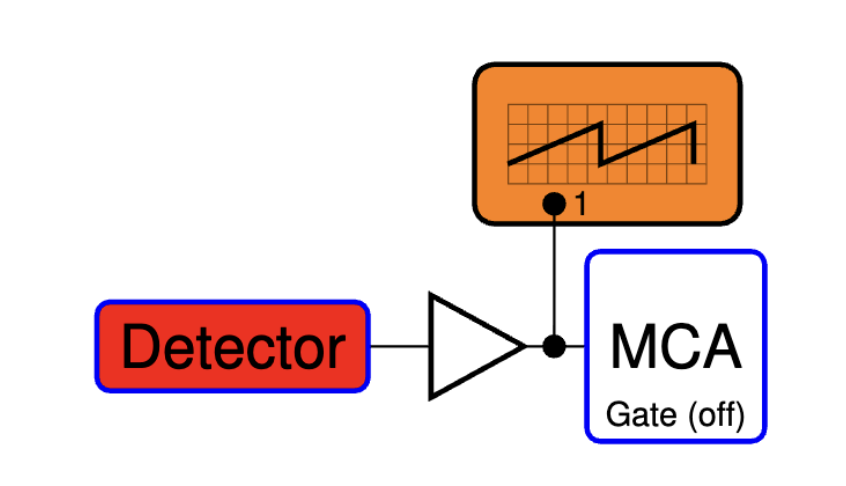
\includegraphics[width=0.5\linewidth]{../Images/Amp Circuit.png}
    \caption{Circuit Diagram for setting amplifier gain. The triangle represents the amplifier, while the orange box is the oscilloscope which here is receiving a signal in channel 1.~\cite{3}}
    \label{fig:amp_circ_diagram}
\end{figure}

In the experiment, we went about this by manually increasing the amplitude on the two main amplifiers until the visible photopeaks from the signals from both the moving and stationary detector were at the right edge of the MCA screen. Since no external gate signal was being sent to the MCA (with its input being set to `Spectrum' and `Gate' being set to `Off'), we saw the full spectrum of the analog signal. However, before we could increase the amplification to the point where the photopeaks were on the right edge of the MCA plot, the signal began getting saturated (the sine curve plateauing). Hence, we only amplified the signal to just before this occurred, keeping the photopeaks in the MCA screen around the centre of the plots.\\

\begin{multicols}{2}
\begin{figure}[H]
    \centering
    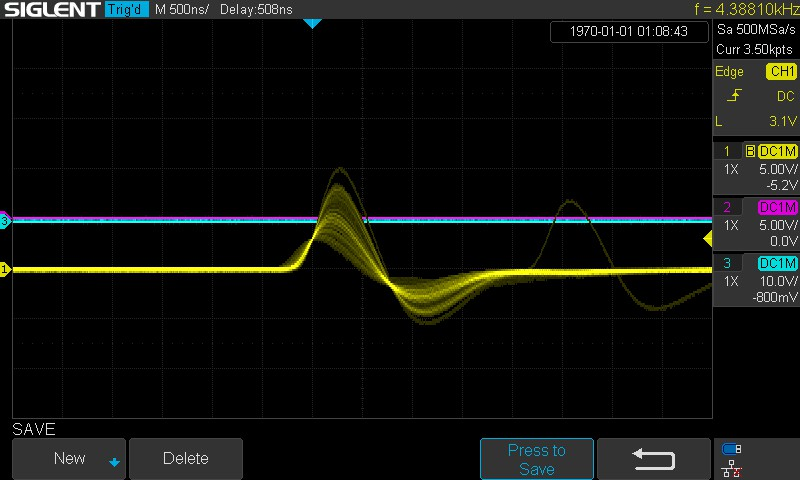
\includegraphics[width=\linewidth]{../Images/SDS00001.jpg}
    \caption{Signal from the moving detector on the oscilloscope}
    \label{fig:oscill_amp_M}
\end{figure}
\begin{figure}[H]
    \centering
    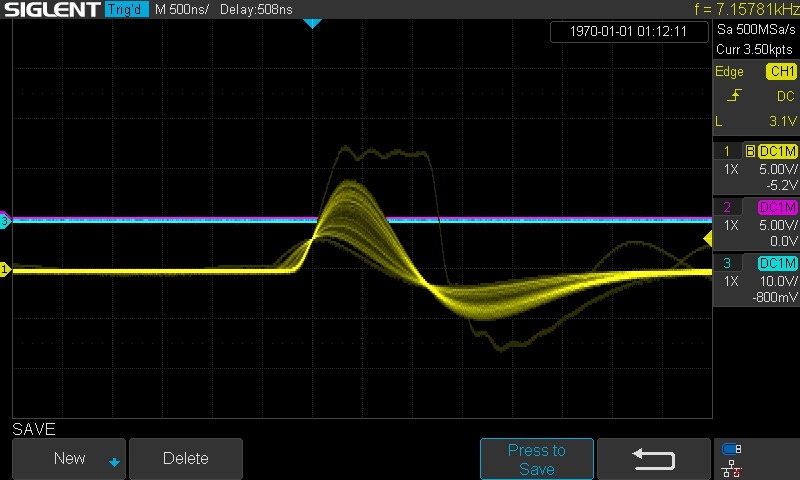
\includegraphics[width=\linewidth]{../Images/SDS00002.jpg}
    \caption{Signal from the stationary detector on the oscilloscope}
    \label{fig:oscill_amp_C}
\end{figure}
\end{multicols}

In the MCA plot of the full spectrum of the signal, we identified two prominent narrow peaks that were close to each other (just before channel 6000 in Fig. \ref{fig:MCA_amp_C}) as the peaks corresponding to the $\gamma-\gamma$ cascade. Since the energies of the associated emitted photons are 1173.2$\,$keV and 1332.5$\,$keV, these peaks seemed good candidates.\\

\begin{figure}[H]
    \centering
    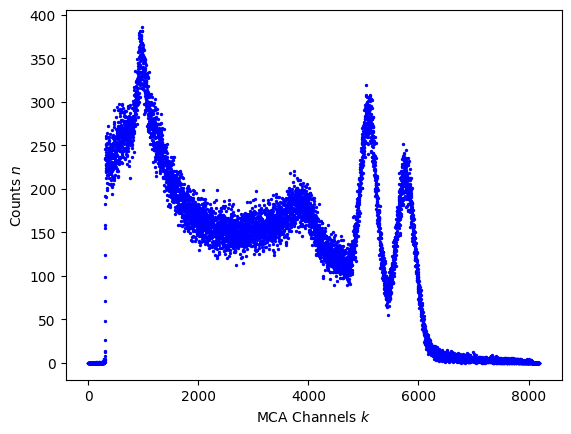
\includegraphics[width=0.6\linewidth]{../Images/Amp Spectrum.png}
    \caption{MCA plot of the spectrum of the analog signal from the stationary detector, after increasing the amplification of the main amplifier.}
    \label{fig:MCA_amp_C}
\end{figure}

\subsection{Calibrating the SCAs}

We next introduced the SCAs into the system. After going through the amplifier, we divided the signal from the detectors into two, sending one through the SCA and then a GDG, while the other was sent through a microsecond delay generator. Both signals were then sent to the oscilloscope and the MCA (see Fig. \ref{fig:sca_circ_diagram}), with the latter having the GDG signal set as its gate (the `Gate' setting now being set to `Coincidence').\\

\begin{figure}[H]
    \centering
    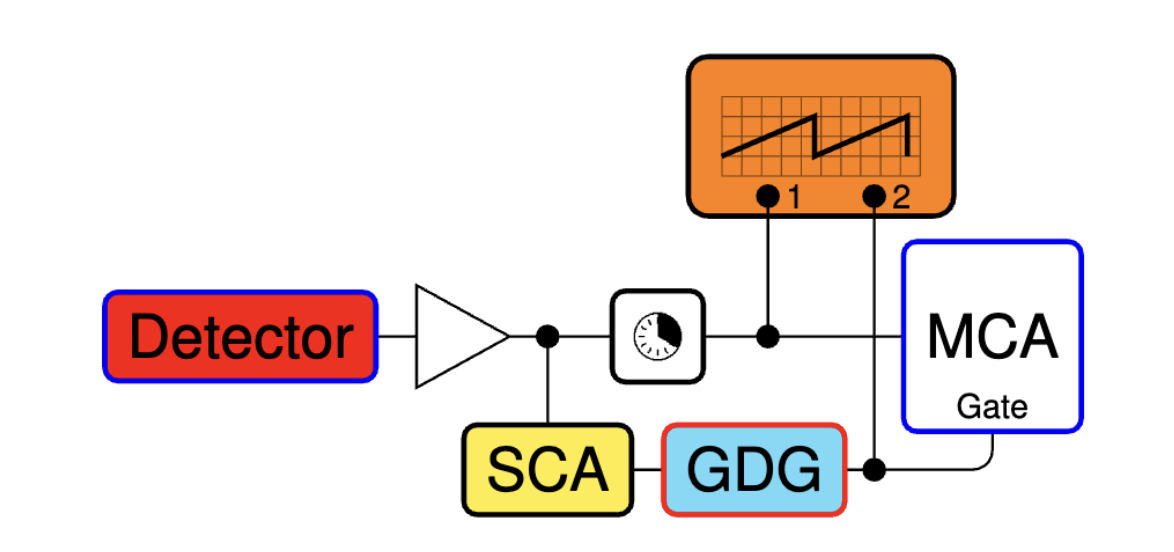
\includegraphics[width=0.6\linewidth]{../Images/SCA Circuit.png}
    \caption{Circuit diagram for calibrating the SCAs. The box with a clock represents a microsecond delay generator.~\cite{3}}
    \label{fig:sca_circ_diagram}
\end{figure}

Using the oscilloscope, we adjusted the microsecond delay such that the analog signal peaks were in between the square wave gate from the GDG (Figs. \ref{fig:oscill_sca_M} and \ref{fig:oscill_sca_C}). Thus, the plot on the MCA showed a cut version of the original spectrum, corresponding to the thresholds set on the SCA. We adjusted these thresholds until only the two photopeaks were fully visible in the energy window (see Figs. \ref{fig:MCA_sca_M} and \ref{fig:MCA_sca_C}). For the moving detector, these thresholds were $6.71\,$V to $8.9\,$V, while for the stationary detector, they were $3.48\,$V to $7.70\,$V. Calculating the sensitivity
$$\eta = \frac{N_{\text{SCA-gated}(E)}}{N_{\text{Self-gated}(E)}}$$
and plotting this too with the spectra shows us that the sensitivity is approximately 100$\%$ around the photopeaks.\\

\begin{multicols}{2}
\begin{figure}[H]
    \centering
    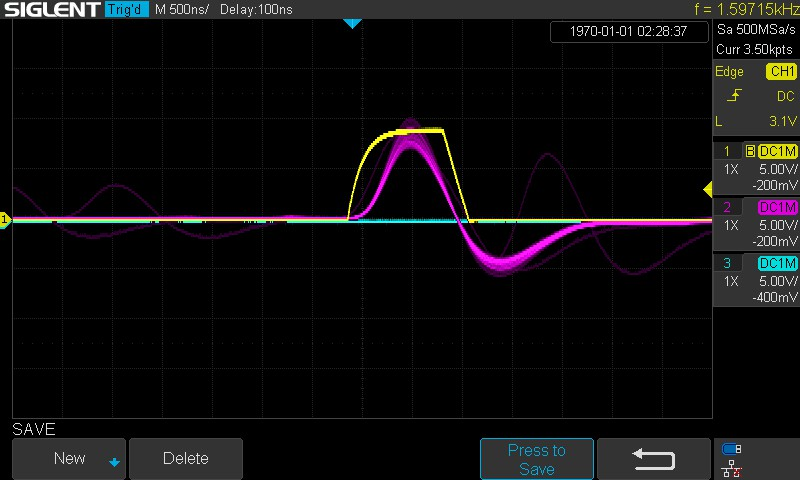
\includegraphics[width=\linewidth]{../Images/SDS00004.jpg}
    \caption{Analog signal from the moving detector on the oscilloscope (pink) with the digital signal from the SCA (yellow); the two coincide}
    \label{fig:oscill_sca_M}
\end{figure}
\begin{figure}[H]
    \centering
    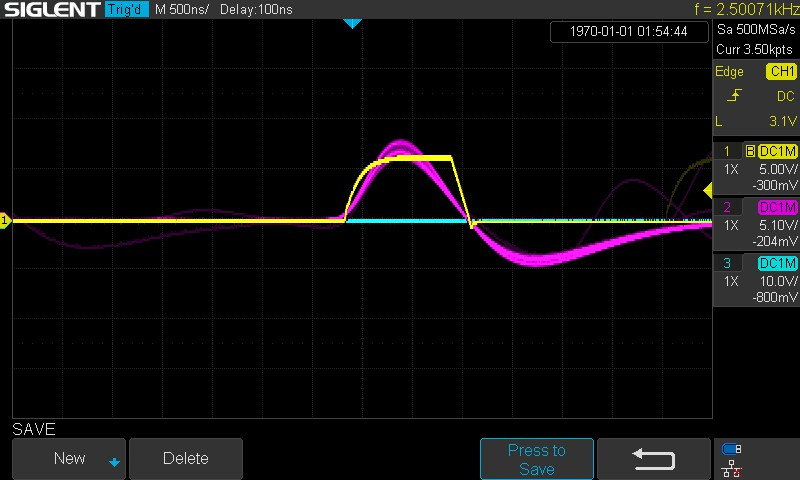
\includegraphics[width=\linewidth]{../Images/SDS00003.jpg}
    \caption{Analog signal from the stationary detector on the oscilloscope (pink) with the digital signal from the SCA (yellow); the two coincide}
    \label{fig:oscill_sca_C}
\end{figure}
\end{multicols}

\begin{multicols}{2}
\begin{figure}[H]
    \centering
    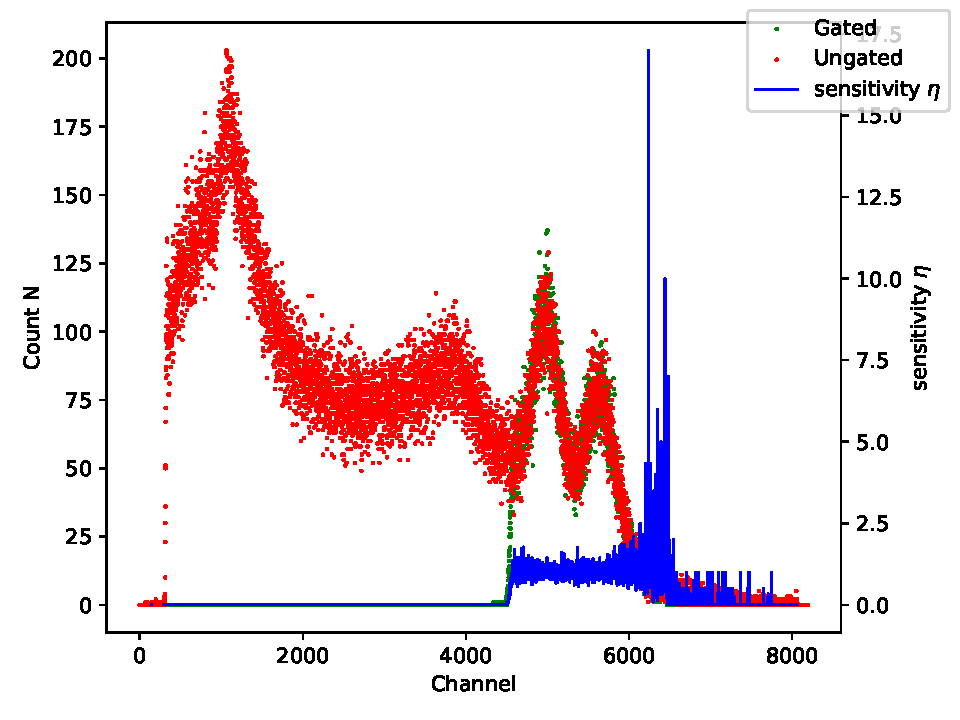
\includegraphics[width=\linewidth]{../Images/SCA_Calib_M.pdf}
    \caption{MCA plot of the spectra of the moving detector's signal, showing the full ungated spectrum, the gated (by SCA) cut spectrum, and the sensitivity.}
    \label{fig:MCA_sca_M}
\end{figure}
\begin{figure}[H]
    \centering
    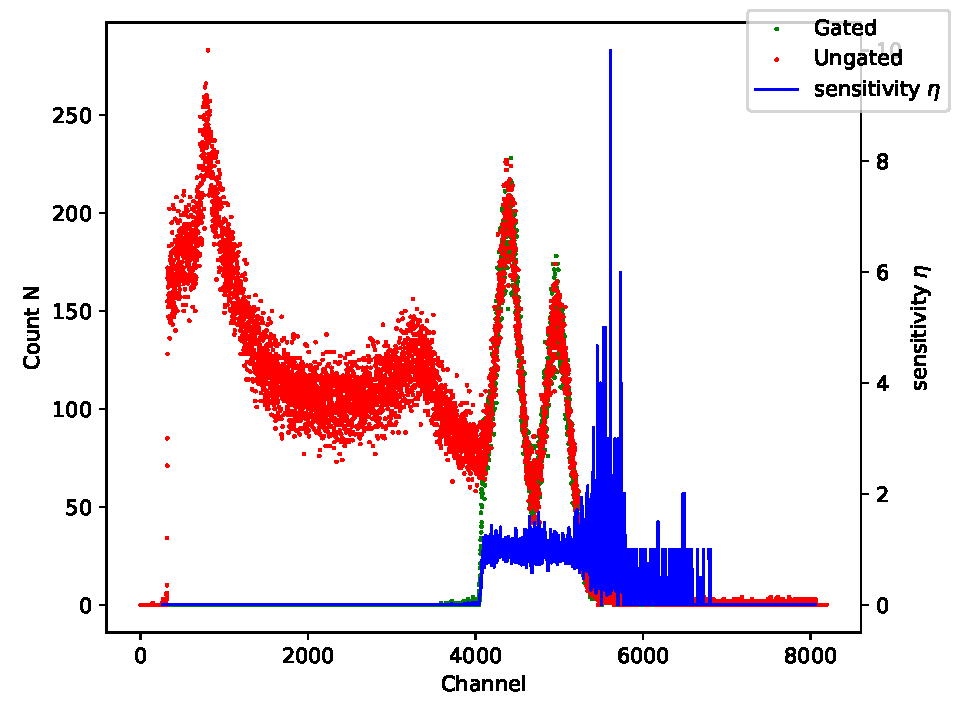
\includegraphics[width=\linewidth]{../Images/SCA_Calib_C.pdf}
    \caption{MCA plot of the spectra of the stationary detector's signal, showing the full ungated spectrum, the gated (by SCA) cut spectrum, and the sensitivity.}
    \label{fig:MCA_sca_C}
\end{figure}
\end{multicols}

% \begin{figure}[H]
%     \centering
%     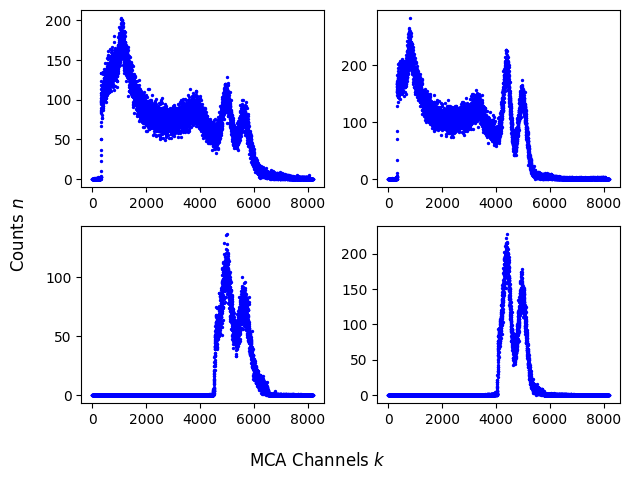
\includegraphics[width=0.8\linewidth]{Images/SCA Spectra.png}
%     \caption{MCA plots of the spectra of the analog signals. The left subplots show data from the moving detector while the right subplots show data from the stationary detector. The top subplots show the entire spectra (i.e. MCA Gate set to `Off') while the bottom subplots show the cut spectra after the SCA-GDG gate was used.}
%     \label{fig:MCA_SCAs}
% \end{figure}

\subsection{Calibrating the CFDs}

After this, we introduced the CFDs to our circuit, splitting the original signal into two, one going via an amplifier to a microsecond delay generator, and another going via an inverse amplifier to a CFD and then a GDG. Both signals were then sent to an oscilloscope and MCA, with the MCA again using the latter signal as a gate (Fig. \ref{fig:cfd_circ_diagram}).\\

\begin{figure}[H]
    \centering
    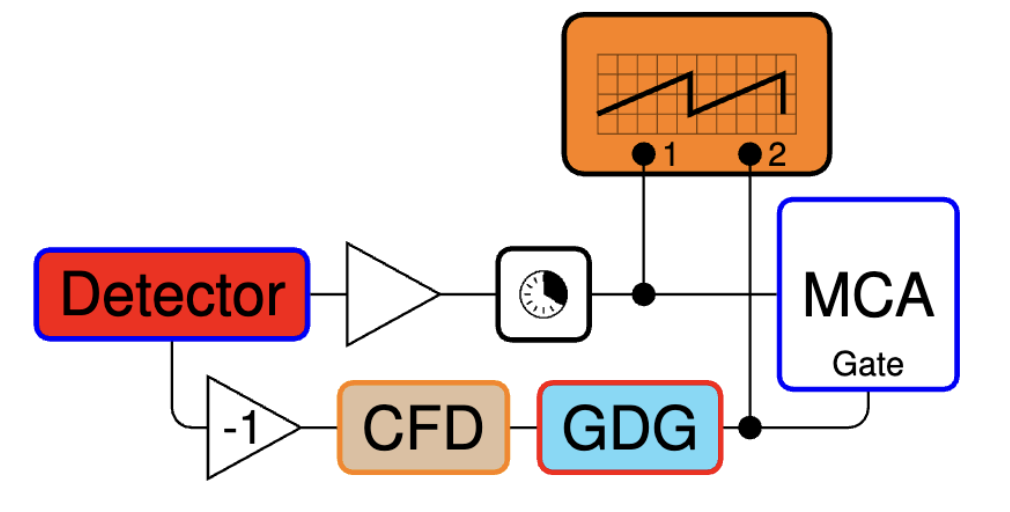
\includegraphics[width=0.6\linewidth]{../Images/CFD Circuit.png}
    \caption{Circuit diagram for calibrating the CFDs. The triangle with a -1 in it represents the inverse amplifier.~\cite{3}}
    \label{fig:cfd_circ_diagram}
\end{figure}

Again, as with the SCAs, we adjusted the delay until the analog part of the signal sat within the square gate (Figs. \ref{fig:oscill_cfd_M} and \ref{fig:oscill_cfd_C}). We also adjusted the thresholds of the CFDs until only the two photopeaks from the original spectrum remained on the MCA (see Figs. \ref{fig:MCA_cfd_M} and \ref{fig:MCA_cfd_C}). Calculating the sensitivity
$$\eta = \frac{N_{\text{SCA-gated}(E)}}{N_{\text{Self-gated}(E)}}$$
and plotting this too with the spectra shows us that the sensitivity is approximately 100$\%$ around the photopeaks.\\

\begin{multicols}{2}
\begin{figure}[H]
    \centering
    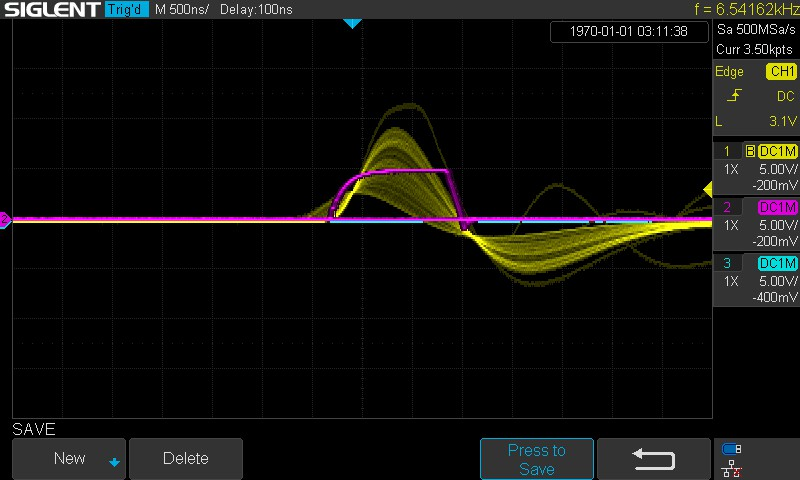
\includegraphics[width=\linewidth]{../Images/SDS00007.jpg}
    \caption{Analog signal from the moving detector on the oscilloscope (pink) with the digital signal from the CFD (yellow); the two coincide}
    \label{fig:oscill_cfd_M}
\end{figure}
\begin{figure}[H]
    \centering
    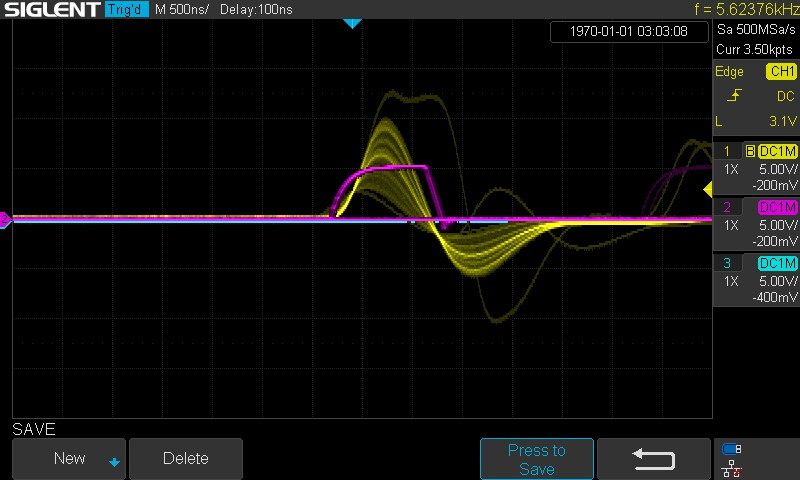
\includegraphics[width=\linewidth]{../Images/SDS00005.jpg}
    \caption{Analog signal from the stationary detector on the oscilloscope (pink) with the digital signal from the CFD (yellow); the two coincide}
    \label{fig:oscill_cfd_C}
\end{figure}
\end{multicols}

\begin{multicols}{2}
\begin{figure}[H]
    \centering
    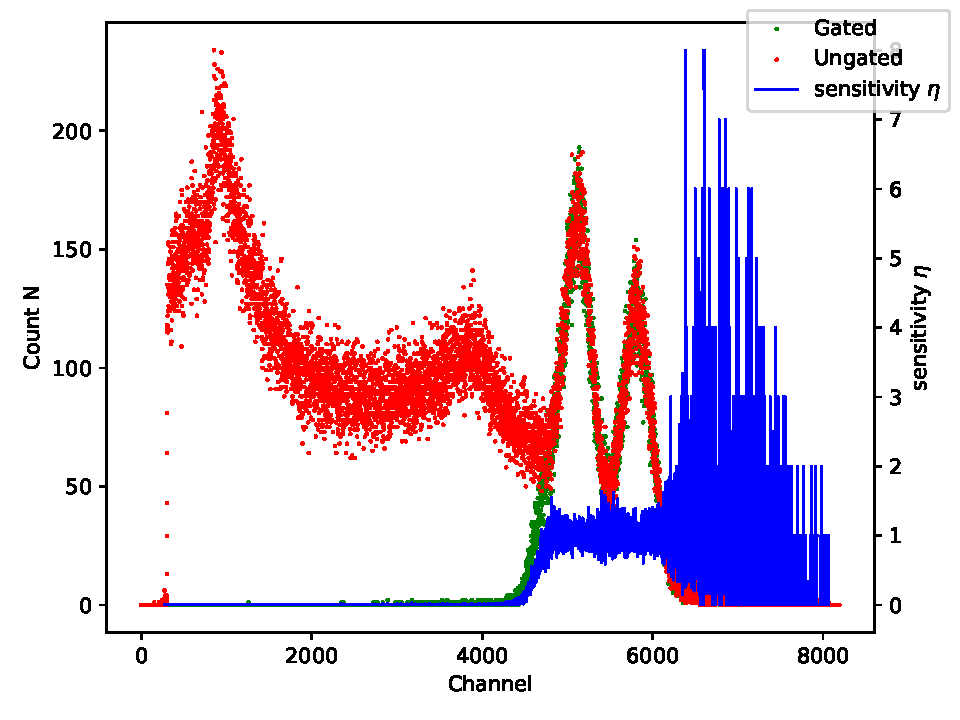
\includegraphics[width=\linewidth]{../Images/CFD_Calib_M.pdf}
    \caption{MCA plot of the spectra of the moving detector's signal, showing the full ungated spectrum, the gated (by CFD) cut spectrum, and the sensitivity.}
    \label{fig:MCA_cfd_M}
\end{figure}
\begin{figure}[H]
    \centering
    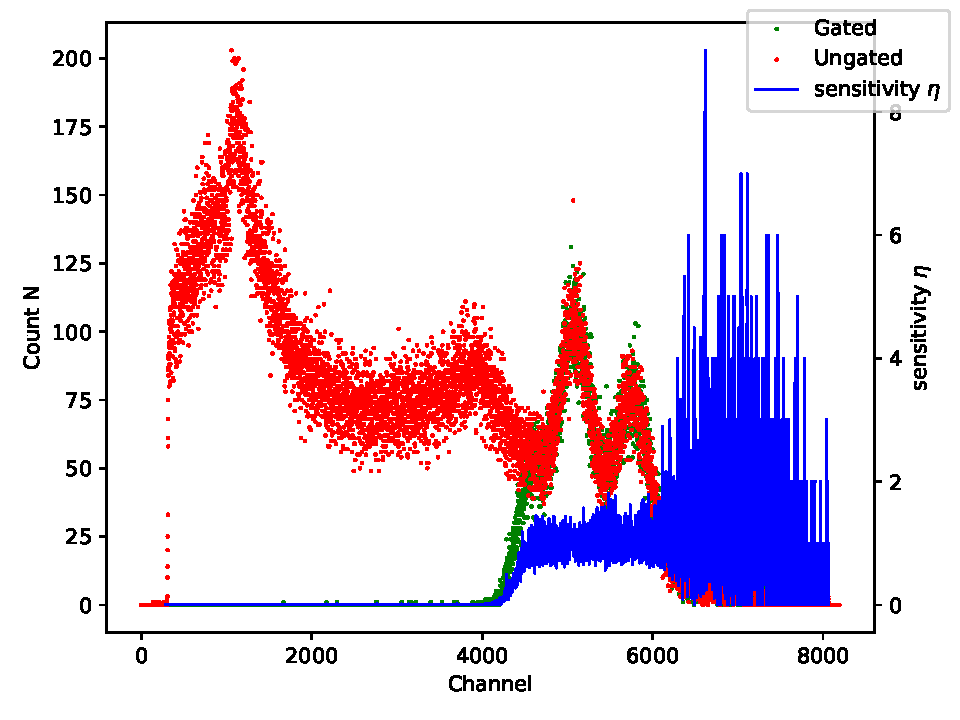
\includegraphics[width=\linewidth]{../Images/CFD_Calib_C.pdf}
    \caption{MCA plot of the spectra of the stationary detector's signal, showing the full ungated spectrum, the gated (by CFD) cut spectrum, and the sensitivity.}
    \label{fig:MCA_cfd_C}
\end{figure}
\end{multicols}

% \begin{figure}[H]
%     \centering
%     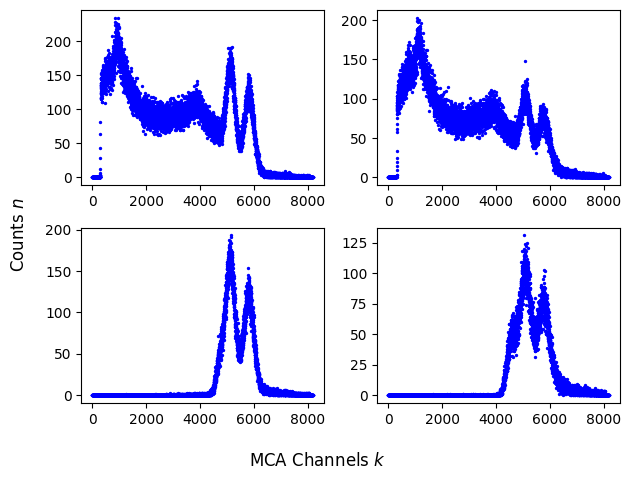
\includegraphics[width=0.8\linewidth]{../Images/CFD Spectra.png}
%     \caption{MCA plots of the spectra of the analog signals. The left subplots show data from the moving detector while the right subplots show data from the stationary detector. The top subplots show the entire spectra (i.e. MCA Gate set to `Off') while the bottom subplots show the cut spectra after the CFD-GDG gate was used.}
%     \label{fig:MCA_CFDs}
% \end{figure}

\subsection{Adjusting the Delay in the Fast Branch}

So far, we had been doing the calibrations for each detector one at a time. We now brought them both into the circuit, sending their signals via inverse amplifiers to CFDs and then to nanosecond delay generators. From here, both signals were split, with one part being sent to the oscilloscope and the other being sent through the fast-coincidence to counter 4 of the MCA (Fig. \ref{fig:fast_circ}).\\

\begin{figure}[H]
    \centering
    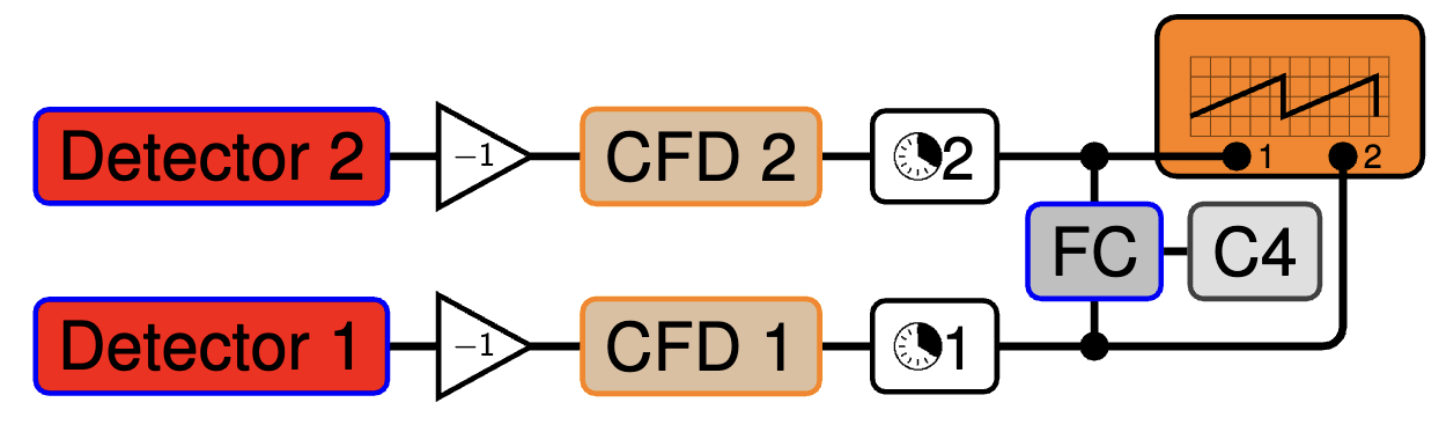
\includegraphics[width=0.6\linewidth]{../Images/Fast Circuit.png}
    \caption{Circuit Diagram for adjusting the fast branch delay. The two delay generators here are nanosecond generators, the box labelled `FC' is a fast-coincidence, and the box labelled `C4' is Counter 4 of the MCA into which the signal is sent.~\cite{3}}
    \label{fig:fast_circ}
\end{figure}

We set the delay of the moving detector to be fixed at $32\,$ns and varied the delay of the stationary detector in the range of $1\,$ns to $63\,$ns in integer steps (i.e. an overall delay between the two signals of $-31$ to $31\,$ns). For each value of the difference in delays, we measured the number of counts recorded by the MCA in 10 seconds.\\

\begin{figure}[H]
    \centering
    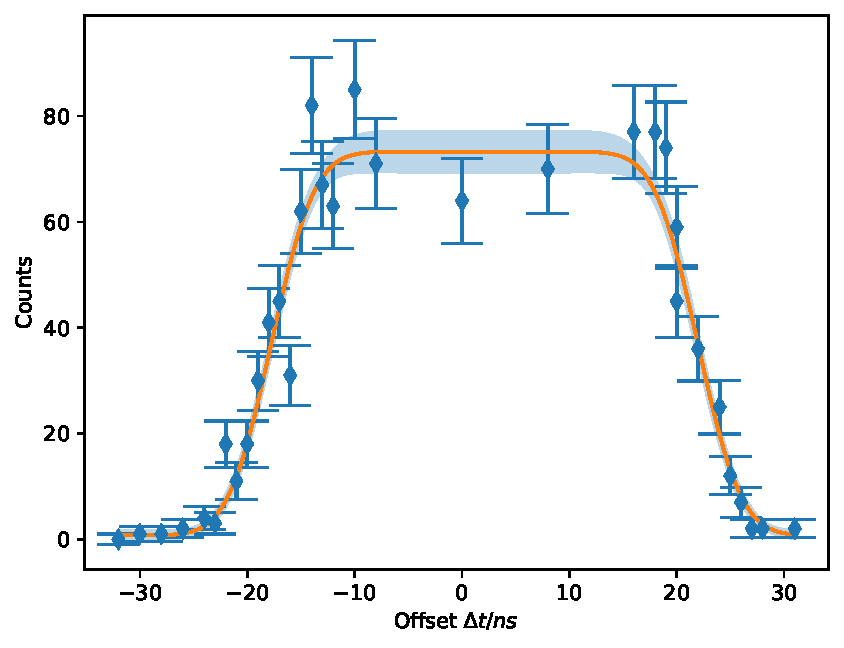
\includegraphics[width=0.7\linewidth]{../Images/prompt_curve.pdf}
    \caption{Prompt Curve from the Fast Branch, with experimental data and uncertainties in blue, and fit in yellow}
    \label{fig:prompt}
\end{figure}

The offset v/s counts data should follow the function
$$f(t) = \frac{A}{2} \cdot \left( 1 + \text{erf}\left( \frac{t-(t_0-\frac{w}{2})}{\sigma} \right) \cdot \text{erf}\left( \frac{(t_0+\frac{w}{2})-t}{\sigma} \right) \right) + A_0$$
where $t$ is the time offset, $A$ is a scaling factor, $A_0$ is the vertical offset on the plot, $\sigma$ is the width of the slopes, $w$ is the resolving time which controls the width of the function, and $t_0$ is the centre of the plateau of the function. The erf function is the Gauss error function
$$\text{erf}(z) = \frac{2}{\sqrt{\pi}} \int_0^z e^{-t^2} dt$$\\

Changing the resolving time changes the width of the plateau, shortening or lengthening it as the resolving time decreases or increases. Having too short a resolving time would not be advantageous as there would only be a small window of delay offsets where we could expect to see a significant number of true coincidences. Having too long a resolving time would also be disadvantageous as now the window where we can measure random coincidences is too small. As can be seen from our plot above, the resolving time we had was just right for the purposes of this experiment. The values of the various parameters from doing the fit are as follows:
\begin{table}
    \centering
    \begin{tabular}{cc}
        \hline
        Parameter & Fit Value \\
        \hline
        $A$ & $72.3 \pm 3.7$ \\
        $A_0$ & $0.66 \pm 0.61$ \\
        $\sigma$ & $4.44 \pm 0.42\,$s \\
        $w$ & $39.71 \pm 0.68\,$s \\
        $t_0$ & $2.07 \pm 0.18\,$s \\
        \hline
    \end{tabular}
    \caption{Values of the Parameters as calculated by the fit}
    \label{tab:fitvals}
\end{table}

\subsection{Adjusting the Delay in the Slow Branch}

As the last step of the calibration before taking the main measurements, we brought in the slow branch to our circuit too (Fig. \ref{fig:slow_circ}). We adjusted the microsecond delays and the GDG delay, along with the widths of the square wave gates to ensure that all three coincided, aligning their edges.\\

\begin{figure}[H]
    \centering
    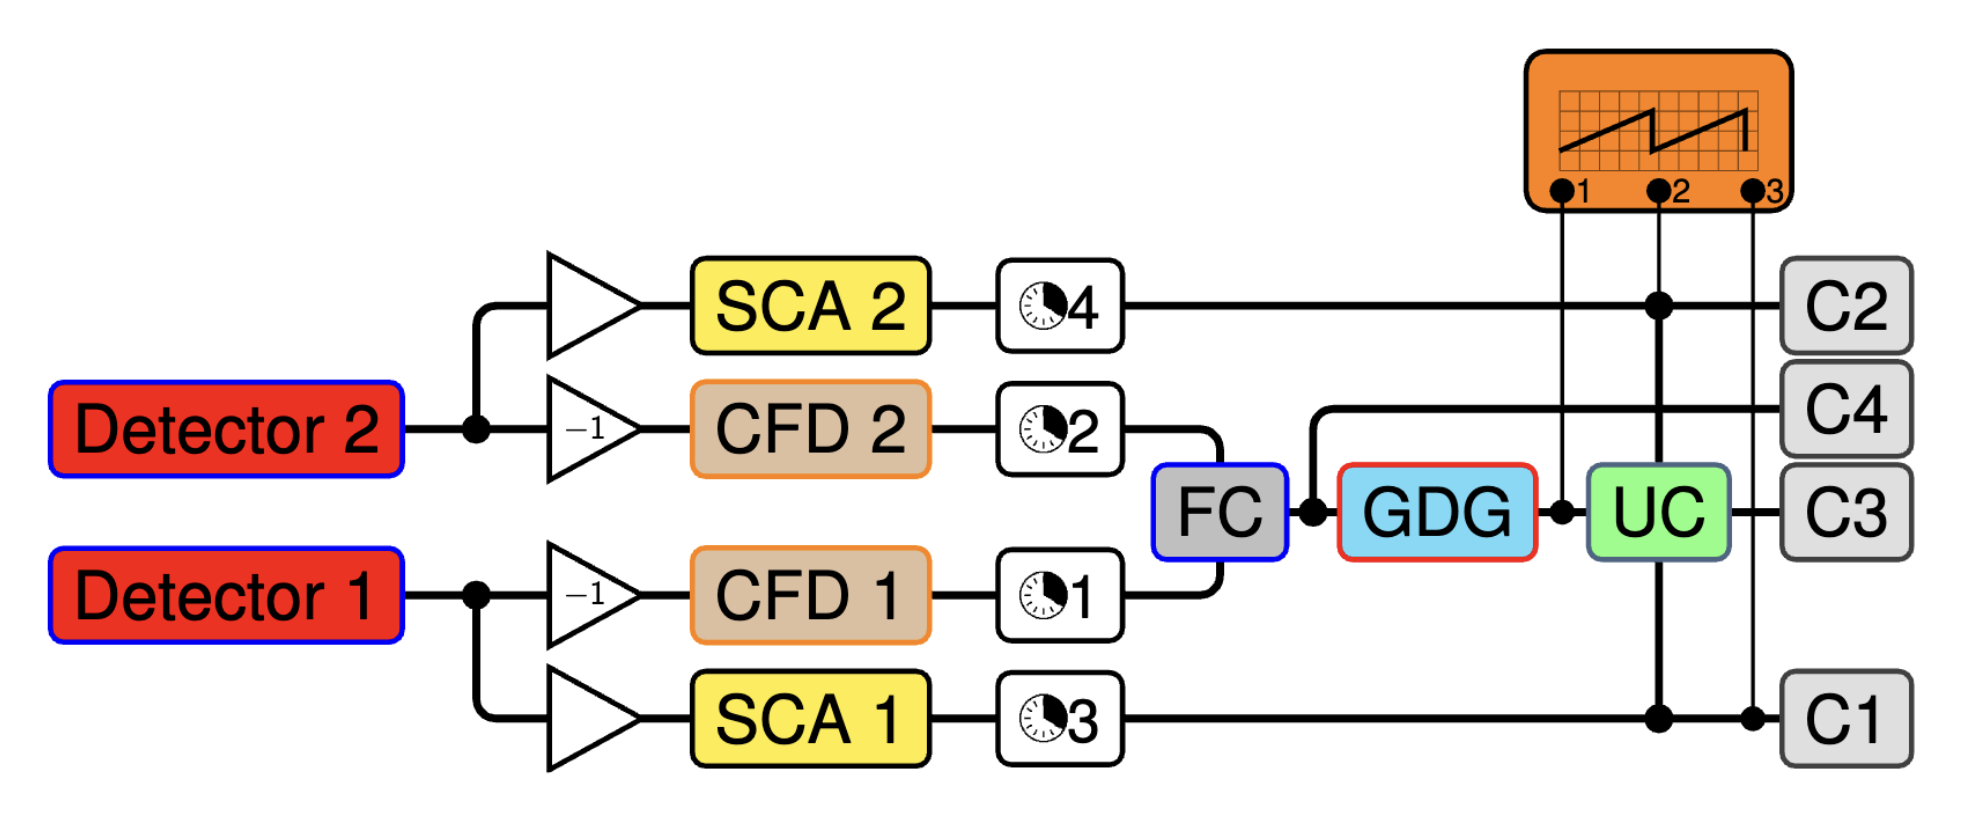
\includegraphics[width=0.7\linewidth]{../Images/Slow Circuit.png}
    \caption{Circuit Diagram for adjusting the slow branch delay. The delay generators labelled 1 and 2 are nanosecond delay generators, while those labelled 3 and 4 are microsecond delay generators. The box labelled `UC' is the universal coincidence, and the boxes labelled `C1' to `C4' are Counters 1 to 4 of the MCA.~\cite{3}}
    \label{fig:slow_circ}
\end{figure}

\begin{figure}[H]
    \centering
    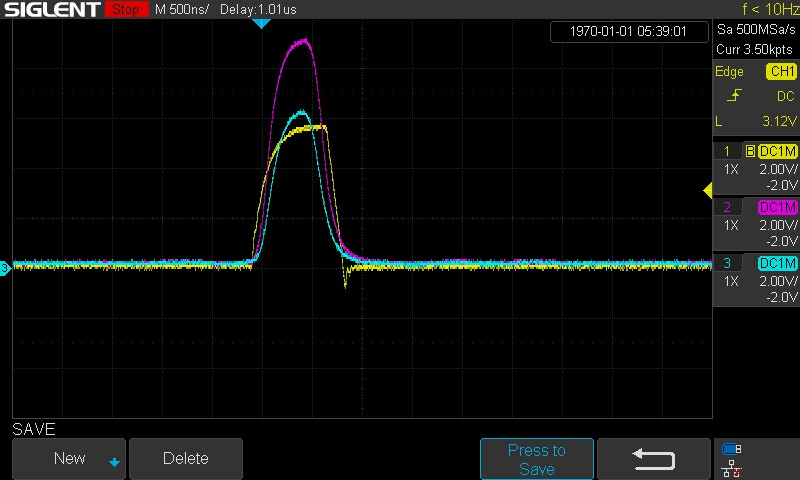
\includegraphics[width=0.7\linewidth]{../Images/SDS00008.jpg}
    \caption{Digital signals from the slow branch on the oscilloscope, with the fast branch gate in yellow, the SCA gate from the stationary detector in pink, and the SCA gate from the moving detector in blue.}
    \label{fig:oscillo_slow}
\end{figure}
